\section{Simulation study}
\label{sim}

We apply the hierarchical model to simulations from a max-autoregressive process. Choose $\theta_i\in(0,1]$ for $i=1,\ldots,R$. Let $W_{i,1}\ldots,W_{i,n}$ be independent unit Fr{\'e}chet random variables, and define
\begin{align}
Y_{i,1} &= W_{i,1}/\theta_i \nonumber \\
Y_{i,j} &= \max\{(1-\theta_i)Y_{i,j-1}, W_{i,j}\}~~~~~j=2,\ldots,n \label{max}
\end{align}
then $Y_{i,\cdot}$ is stochastic process having extremal index $\theta_i$. We let $R=10$, $n=1000$, and $\theta_1=\cdots=\theta_R$.

Comparisons between models (\ref{ferro}) and (\ref{suveges}) are made using coverage and RMSE.

% \begin{figure}
% 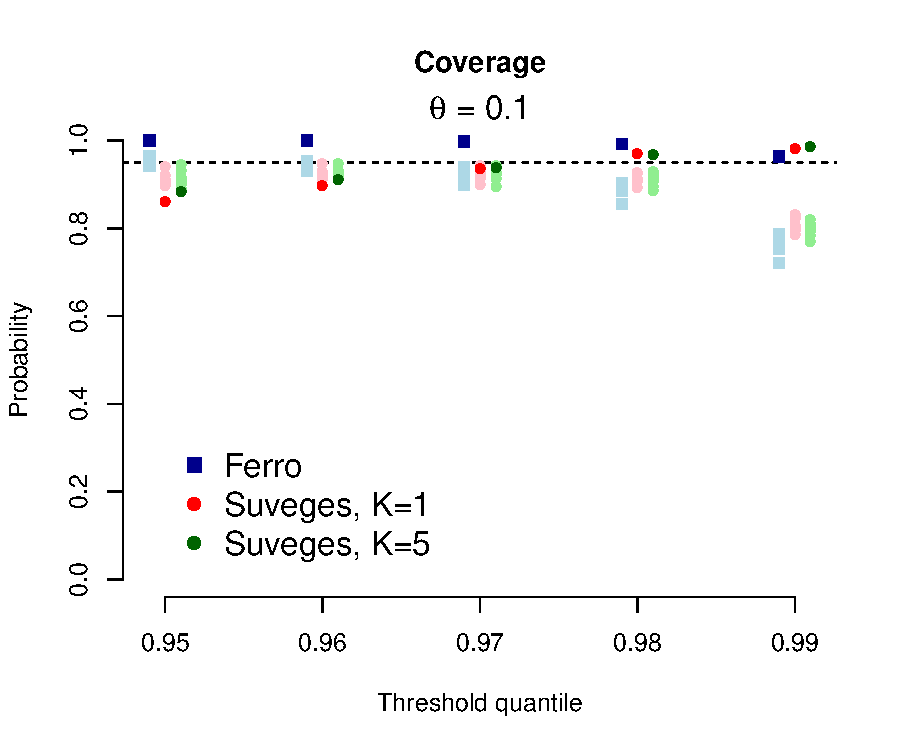
\includegraphics[scale=0.49]{../extremal_comparison/figs/sim_coverage_10.pdf}
% 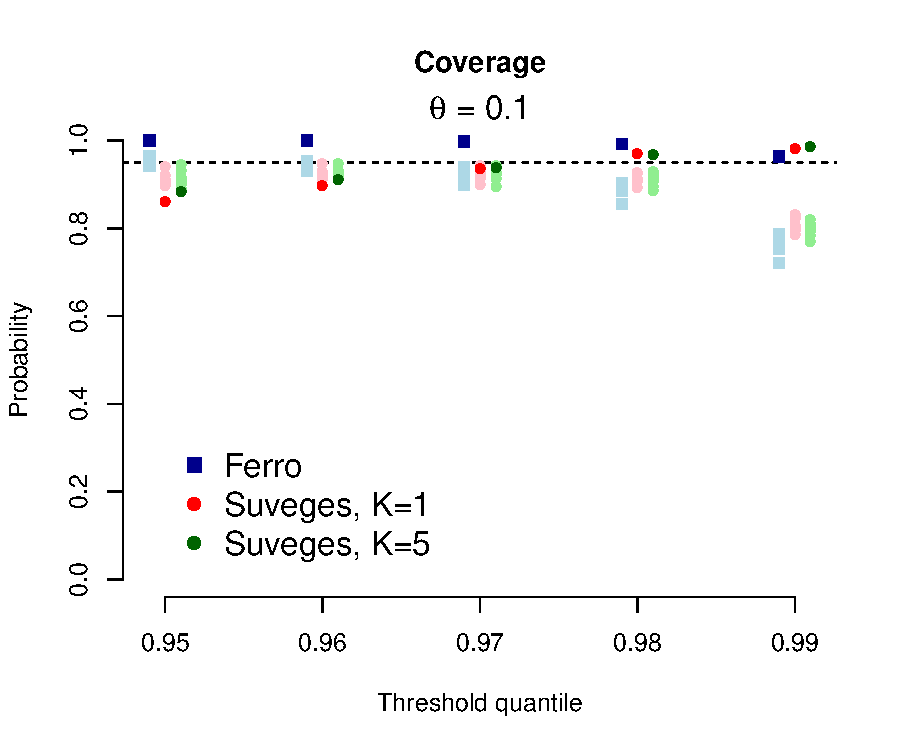
\includegraphics[scale=0.49]{../extremal_comparison/figs/sim_coverage_10.pdf}
% 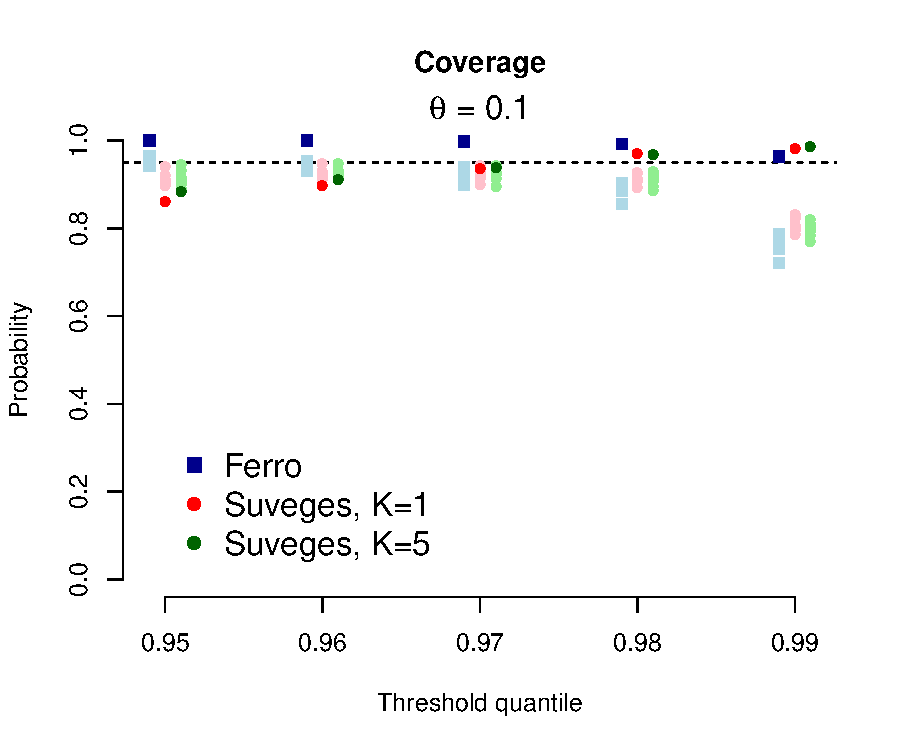
\includegraphics[scale=0.49]{../extremal_comparison/figs/sim_coverage_10.pdf}
% \end{figure}
% 
% \begin{figure}
% 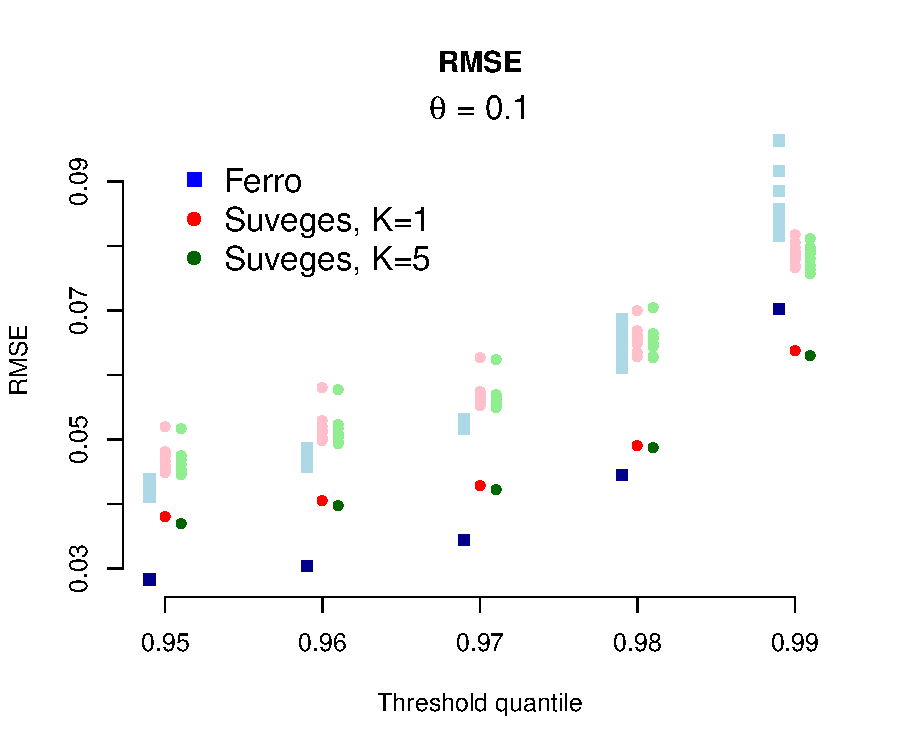
\includegraphics[scale=0.3]{../extremal_comparison/figs/sim_rmse_10.pdf}
% 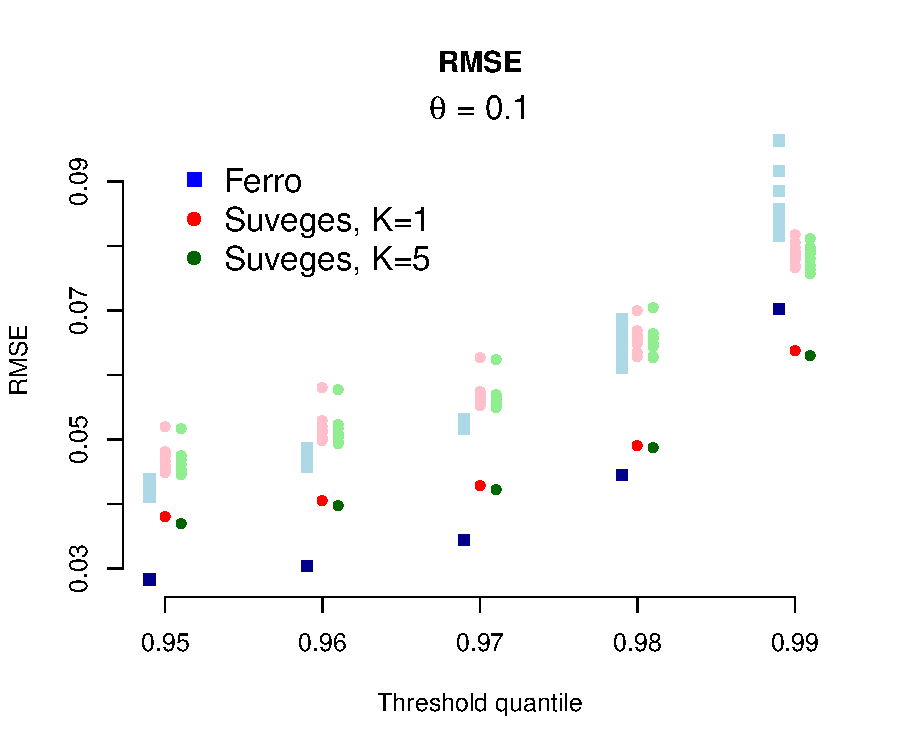
\includegraphics[scale=0.3]{../extremal_comparison/figs/sim_rmse_10.pdf}
% 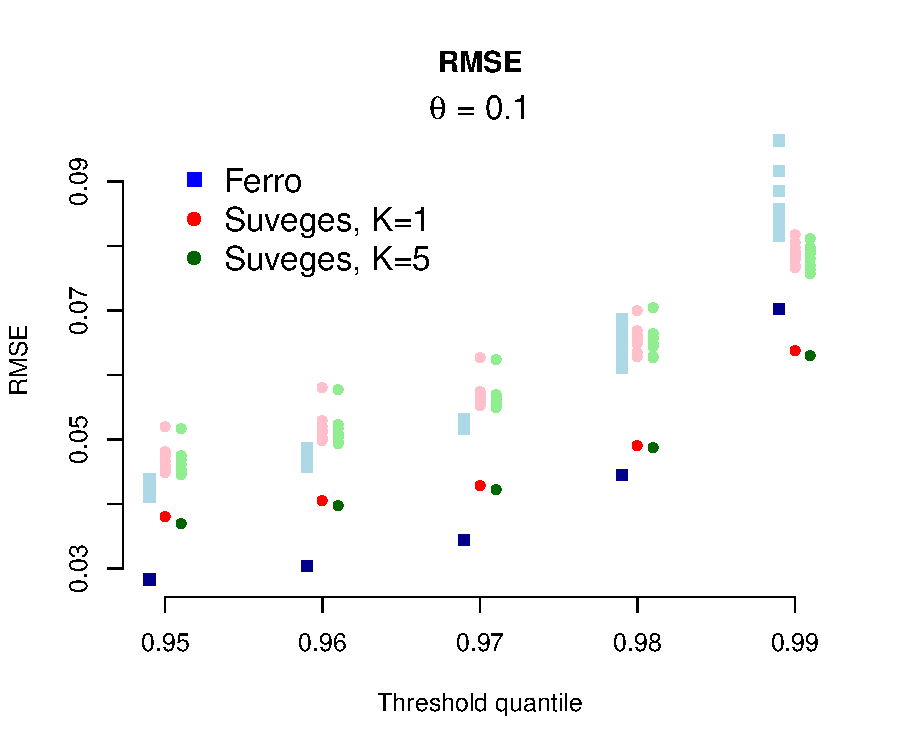
\includegraphics[scale=0.3]{../extremal_comparison/figs/sim_rmse_10.pdf}
% \end{figure}

\begin{figure}
\begin{center}
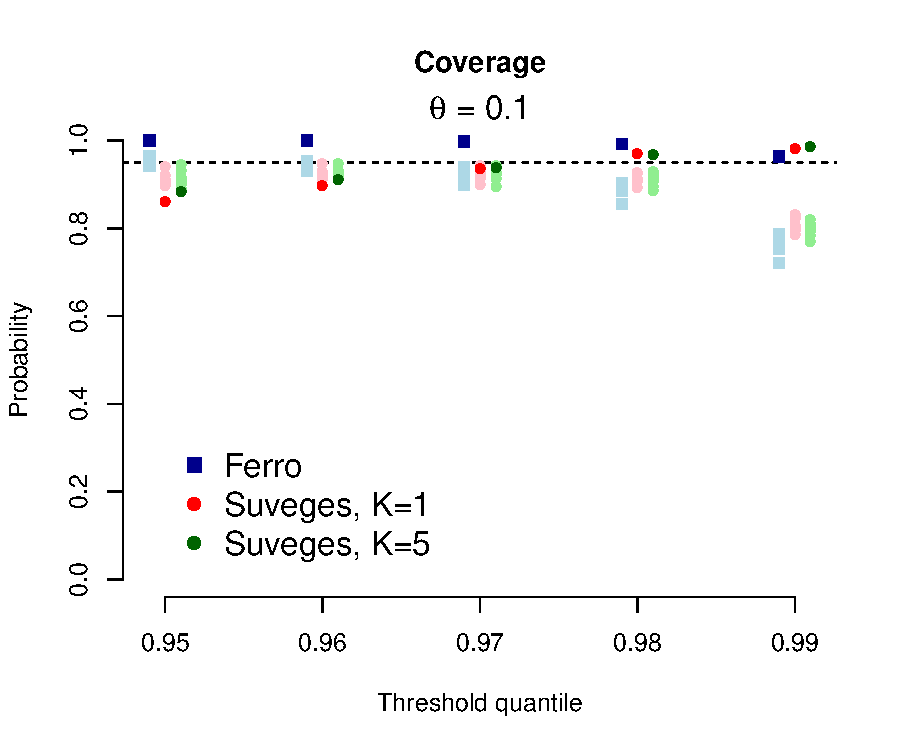
\includegraphics[scale=0.48]{../extremal_comparison/figs/sim_coverage_10.pdf}
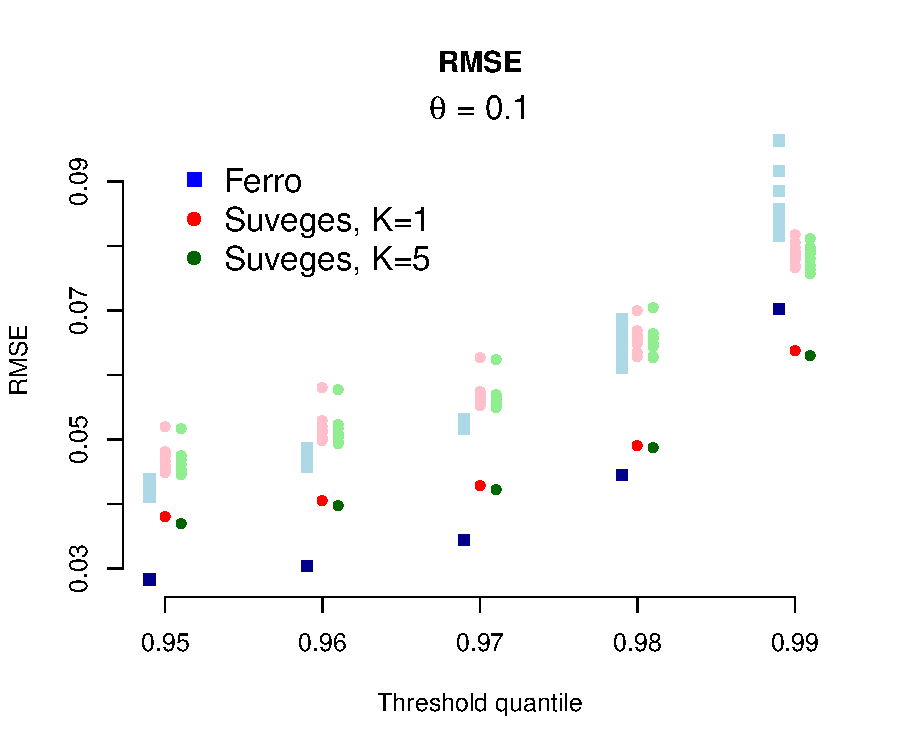
\includegraphics[scale=0.48]{../extremal_comparison/figs/sim_rmse_10.pdf}
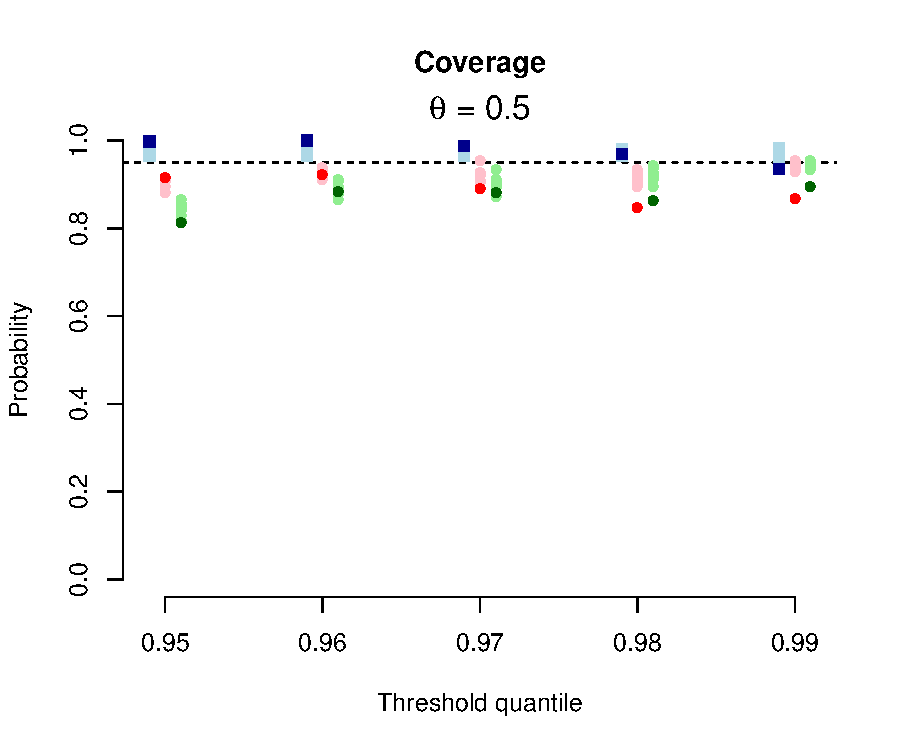
\includegraphics[scale=0.48]{../extremal_comparison/figs/sim_coverage_50.pdf}
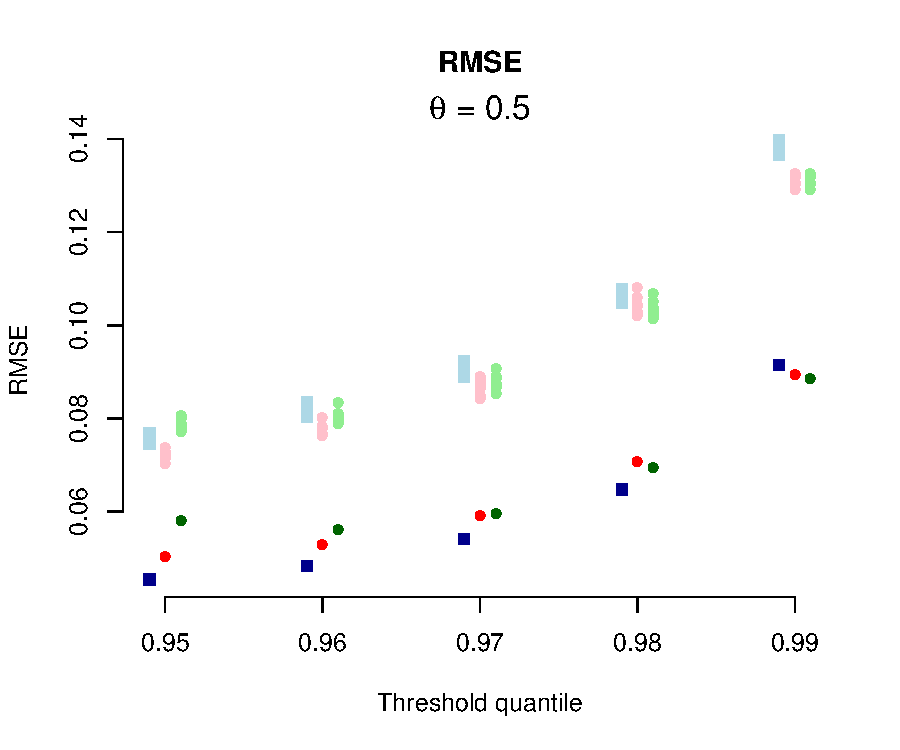
\includegraphics[scale=0.48]{../extremal_comparison/figs/sim_rmse_50.pdf}
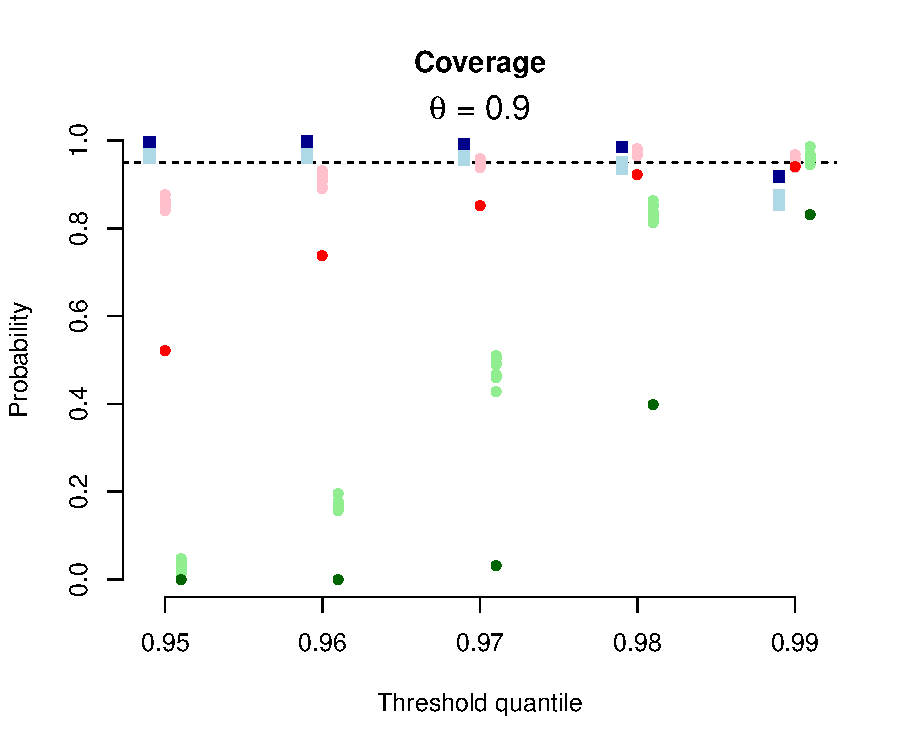
\includegraphics[scale=0.48]{../extremal_comparison/figs/sim_coverage_90.pdf}
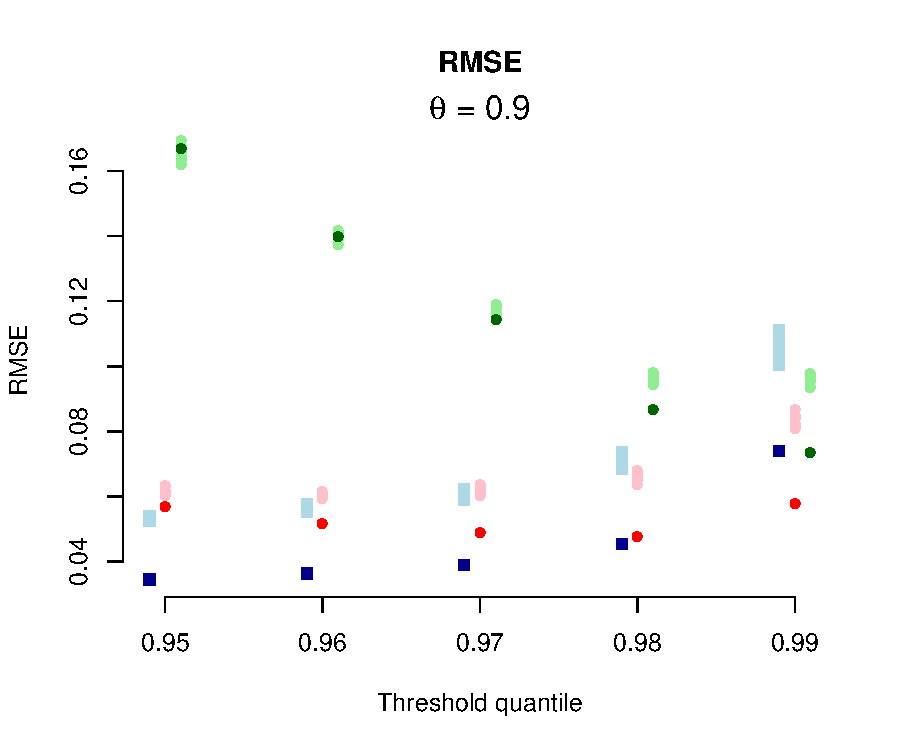
\includegraphics[scale=0.48]{../extremal_comparison/figs/sim_rmse_90.pdf}
\end{center}
\caption{Coverage (left column) and RMSE (right) for the two likelihoods in the simulation study. Each row is based on a different extremal index, either $0.10$, $0.50$, or $0.90$. The darker points represent the hierarchical mean, the lighter points are from the individual sequences. The nominal coverage probability (0.95) is marked by the dashed horizontal line.}
\label{simfigs}
\end{figure}
